\chapter{Container-Runtimes}
\label{chap:compCtnrRuntimes}

Container-Runtimes sind das Herz eines jeden Container-Angebots. Sie laden benötigte Images herunter und instanziieren übergebene Prozesse in Containern. In diesem Kapitel werden verschiedene Runtimes miteinander verglichen und veranschaulicht, wie Runtimes neben Docker für spezielle Anforderungen geeignet sind.

\section{Vorgehen}
\label{sec:vorgehen}
Um verschiedene Runtimes zu vergleichen wurde eine eigene Anwendung mit drei Microservices implementiert. Dabei wurden, wie in \fref{fig:todosStack} zu sehen, verschiedene Technologien verwendet, um zu prüfen, wie die getesteten Container-Runtimes mit diesen umgehen. Diese wurde im Folgenden mit verschiedenen Runtimes bereitgestellt.

\begin{figure}[h]
	\begin{center}
		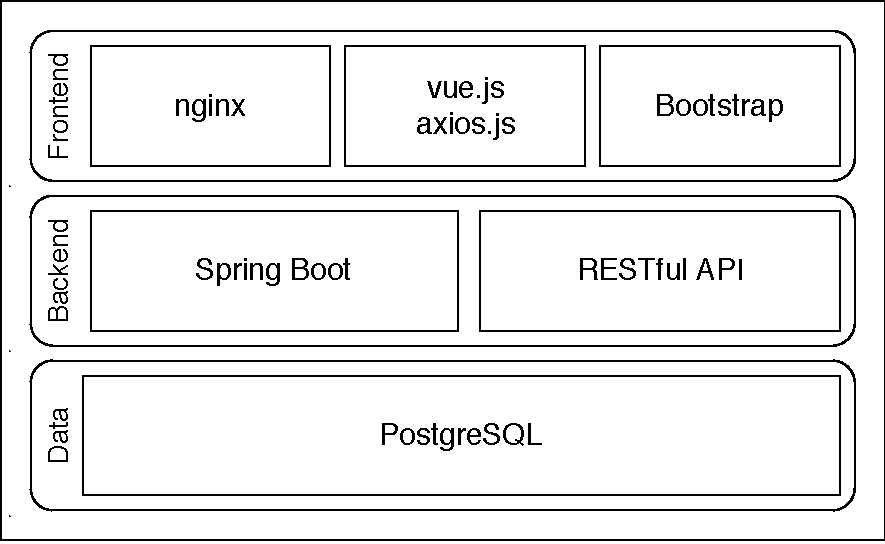
\includegraphics[width=0.7\textwidth]{bilder/microservice-example-stack.pdf}
		\caption{Beispielhafte Darstellung einer Micorservice-Architektur}
		\label{fig:todosStack}
	\end{center}
\end{figure}

\section{Docker Stack}
\label{sec:compDocker}
Docker ist der De-Facto-Standard unter den Container-Technologien. Dabei wird Docker im gesamten \gls{acr-dtap}-Zyklus verwendet.

Notes:
\begin{itemize}
	\item Docker hub / Docker Store einfach zu nutzen
	\item gedacht für Apps
	\item großes Angebot an Images (Hub)
	\item Docker compose
	\item kein extra Tooling
	\item Netzwerk offen, einfach für Testen, unsicherer
	\item Stack komplex, Debuggen schwieriger
	\item nahezu überall genutzt, CRI-O / CRI-Contaienrd in Kubernets
	\item Security Probleme "Running other Code as root"
	\item run everything as root, root benötigt für vieles
\end{itemize}

\section{rkt}
\label{sec:compRkt}
Notes
\begin{itemize}
	\item Installation durch shell script (provided durch CoreOS) oder durch bauen der bin von github repos
	\item unixesque CLI
	\item kein Zentraler Deamon, dadurch integrierbar in init system
	\item gedacht um einzelne Apps zu deployen, nicht ganze Linux Systeme
	\item kaum bis kein wissen über Kernel notwendig
	\item AppC Standard, Docker images, OCI bundles
	\item CNI Networking, CNCF Standard
	\item Secure, crypto validierung default
	\item Jedes Images SOLLTE signiert sein, sichere Quellen
	\item kein root zur laufzeit benötigt
\end{itemize}

\section{LXD / LXC}
\label{sec:compLXD}
Notes:
\begin{itemize}
	\item Installiert auf Ubuntu by Nature
	\item Gedacht für volle Linux Distros, nicht unbedingt Apps
	\item in Verbindung mit Docker, statt direkte Konkurenz
	\item LXD = LXC + RESTful API
	\item Docker bis anfang 2014 based of LXC
	\item komplexer zu nutzen, da lower Level
	\item Network zwischen Containern nur mit Linux mitteln, wissen von Nöten
	\item Betroffen von Linux-Kernel issues, keine Abstarktion
\end{itemize}

\section{runC}
\label{sec:compRunc}

Notes:
\begin{itemize}
	\item OCI stdimpl
	\item Low Level
	\item OCI bundles, mehrere Dateien zur Steuerung (config json, rootfs tar)
	\item Trend zu std, docker impl
	\item keine Versicherung durch Signatur / Verschlüsselung
	\item CRI-O für Kubernets
\end{itemize}

\section{VM basierte Runtimes}
\label{sec:compVMbased}

Notes:
\begin{itemize}
	\item Mehr sicherheit, seperation Kernel
	\item Weniger Performance, Einzelne Aufrufe, starten und stoppen, ... "teurer" 
	\item Erklären KataContaienrs, gVisor (neue Runtime)
\end{itemize}

\todo{gvisor, kata, HyperV Containers, ...}

\section{Fazit}
\label{sec:compFazit}